\documentclass[oneside,
  digital, %% This option enables the default options for the
           %% digital version of a document. Replace with `printed`
           %% to enable the default options for the printed version
           %% of a document.
  table,   %% Causes the coloring of tables. Replace with `notable`
           %% to restore plain tables.
  nolof,     %% Prints the List of Figures. Replace with `nolof` to
           %% hide the List of Figures.
  nolot,     %% Prints the List of Tables. Replace with `nolot` to
           %% hide the List of Tables.
  %% More options are listed in the user guide at
  %% <http://mirrors.ctan.org/macros/latex/contrib/fithesis/guide/mu/fi.pdf>.
]{fithesis3}
%% The following section sets up the locales used in the thesis.
\usepackage[resetfonts]{cmap} %% We need to load the T2A font encoding
\usepackage[T1,T2A]{fontenc}  %% to use the Cyrillic fonts with Russian texts.
\usepackage[
  main=english, %% By using `czech` or `slovak` as the main locale
                %% instead of `english`, you can typeset the thesis
                %% in either Czech or Slovak, respectively.
  german, russian, czech, slovak %% The additional keys allow
]{babel}        %% foreign texts to be typeset as follows:
%%
%%   \begin{otherlanguage}{german}  ... \end{otherlanguage}
%%   \begin{otherlanguage}{russian} ... \end{otherlanguage}
%%   \begin{otherlanguage}{czech}   ... \end{otherlanguage}
%%   \begin{otherlanguage}{slovak}  ... \end{otherlanguage}
%%
%% For non-Latin scripts, it may be necessary to load additional
%% fonts:
\usepackage{paratype}
\def\textrussian#1{{\usefont{T2A}{PTSerif-TLF}{m}{rm}#1}}
%%
%% The following section sets up the metadata of the thesis.
\thesissetup{
    university    = mu,
    faculty       = fi,
    type          = mgr,
    author        = Martin Štefanko,
    gender        = m,
    advisor       = {Bruno Rossi, PhD},
    title         = {Use of Transactions within a Reactive Microservices Environment},
    TeXtitle      = {Use of Transactions within a Reactive Microservices Environment},
    keywords      = {transactions, Narayana, JTA, reactive, microservices, asynchronous, saga, compensating transactions},
    TeXkeywords   = {transactions, Narayana, JTA, reactive, microservices, asynchronous, saga, compensating transactions},
}
\thesislong{abstract}{
abstract
}
\thesislong{thanks}{
   thanks
}
%% The following section sets up the bibliography.
\usepackage{booktabs}

\usepackage{makeidx}      %% The `makeidx` package contains
\makeindex                %% helper commands for index typesetting.
%% These additional packages are used within the document:
\usepackage{paralist}
\usepackage{amsmath}
\usepackage{amsthm}
\usepackage{amsfonts}
\usepackage{url}
\usepackage{menukeys}
\usepackage{minted}


\begin{document}
\chapter{Introduction}

\clearpage
\chapter{Transaction concepts}

This chapter introduces the basic notions of transactions, their properties and common problems of the management of transactions across multiple nodes in the distributed systems. 

\section{Transaction}

A transaction is an unit of processing that provides all-or-nothing property to the work that is conducted within its scope, also ensuring that shared resources are protected from multiple users \cite{java_tran_processing}. It represents an unified and inseparable sequence of operations that are either all provided or none of them take effect. 

From the application point of view there exist several transaction models in which the transactions can be executed. The applicable models in the transaction management are local, programmatic and declarative transaction models. All three models will be described in detail in the following section.

The transaction can end in two forms: it can be either \textit{commited} or \textit{aborted}. The commit determines the successful outcome - all operations within the transaction have been performed and their results are permanently stored in a durable storage. The abort means that all performed operations have been undone and the system is in the same state as if the transaction have not been started.

Generally the achieving of above features may differ. The most common pattern for the transaction processing is a two phase commit protocol with the ACID transactions. Other approaches are based on the relaxation of the one or more of ACID properties to adjust to the real world environments.

\section{2PC protocol}

\section{ACID properties}

A transaction can be viewed as a group of business logic statements with certain shared properties \cite{nar_wf}. Generally considered properties are one or more of atomicity, consistency, isolation and durability. These four properties are often referenced as ACID properties \cite{haerder_reuter_1983} and they describe the major points important for the transaction concepts.

\subsection{Atomicity}

The transaction consists of a sequence of operations performed on different resources or by different participants. Atomicity means that all operation in the transaction are performed as if they were a single operation. When the transaction commits successfully all of its participants are also required to perform a valid commit. Conversely, if the transaction fails and is aborted all performed operations and effects are forced to be undone. This defines a possibility to abort at any point so that all changes done by the transaction will be reverted to the state before the transaction start.

The atomicity is generally achieved by the usage of the consensus multi-phase protocols. Standardized protocol is the two phase commit protocol which is used by the majority of modern transaction systems. 

\subsection{Consistency}

The consistency describes that the transaction maintains the consistency of the system and resources that it is performed on. When the transaction is started on the consistent system this system must remain consistent when the transaction ends - it moves from one consistent state to another.

Unlike other transactional properties (A, I, D), consistency cannot be realized by the transaction system as it does not hold any semantic knowledge about the resources it manipulates \cite{java_tran_processing}. Therefore achieving this property is the responsibility of the application code.

\subsection{Isolation}

The isolation property takes effect when multiple transactions can be executed concurrently on the same resources. That means concurrent transactions can not interfere one with another. Therefore each concurrent execution on the shared resource must be equivalent to some serial ordering of contained transactions which is why the isolation is often also referenced as serializability.

From the perspective of an external user the isolation property means that the transaction appears as it was executed entirely by itself. This means that even if there are multiple transactions in the system executed concurrently, this fact is hidden from the every external view.

As an instinctive extension of the consistency property, the serial execution of the transaction keeps the consistent state. The execution of the transactions in parallel therefore cannot result into the inconsistent system.

\subsubsection{Isolation levels}

As transactions were first defined only in the database environment, in practice we distinguish several levels that describe to which extent the isolation succeeds.


\subsection{Durability}

This property characterizes that all changes done by the transactions must be persistent, i. e. any state changes performed during the transaction must be preserved in case of any subsequent system failure. How the state is preserved usually depends on the particular implementation of the transaction system. Generally, to achieve this property the use of the persistent storage like a disk drive or a cloud is sufficient. Even if this kind of storage is acceptable, it still can not prevent data loss in the case of the catastrophic failure.



\section{Transaction models}


\section{Distributed transactions}

A distributed transaction is the transaction performed in a distributed system.  
The distributed system consists of a number of independent devices connected through a communication network. Such systems are liable to the frequent failures of individual participants or communication channels between them. 

The transaction manager can be implemented as a separate service or being placed with some participant or the client. \textbf{TODO}

\section{Transaction manager}

Every transaction is associated with a transaction coordinator or transaction manager which is responsible for the control and supervision of the participants performing individual operations. It is a component liable for coordinating transactions in the sequential or parallel execution across one or more resources. It provides proper and complete execution and it administers the comprehensive result of the transaction.  Applications are commonly required only to contact the transaction manager about the start of the transaction.

The main responsibilities of transaction manager are starting and ending (commit or abort) of the transaction, management of the transaction context, supervision of transactions scoped across multiple resources and the recovery from failure.

\subsection{Local transaction manager}

A local transaction manager or a resource manager is responsible for the coordination of transactions concerning only a single resource. Because of its scope it is often build in directly to the resource. The span of the resource is defined by its managing platform. 

The resource manager is required to provide a support for the participation in the global transactions that span over several resources. This means that it is effectively capable to handle complete transaction processing to the different transaction manager.

\section{Failure handling}





CA CP theorem - CAP



\clearpage
\chapter{Microservices architecture pattern}

This chapter introduces the basic concept of microservices and describes why modern scalable enterprise applications are to be developed implementing this pattern.

\section{Architecture pattern}

Microservices as a subset of a service oriented architecture (SOA) \cite{soa} is an architectural pattern which offers an intuitive approach to common problems following the software development. Instead of the SOA which builds the applications around the logical domain, microservices are built around the business model. Each microservice represents the separated part of the system.

\subsection{Monolithic architecture}

When describing microservices, the common way is to start by defining the opposite pattern, the monolithic architecture. When the application is developed in a monolithic fashion, all of its content is being implemented and deployed as a single archive. Every component, i. e. "a unit of software that is independently replaceable and upgradeable" \cite{microservices}, is tightly coupled with the application, which is using it. Because of the easy development, scalability and deployment of monolithic software this approach is being preferred by the majority of modern enterprise applications. However, when the application needs to be extended or rebuild, it can become difficult to maintain. For instance, even because of the minor change or update in the single component, the scaling and the continuous deployment of the whole application can stagnate. 

\subsection{Microservice architecture}

Microservices introduced the application separation into the self-maintained units – services \cite{intro_to_microservices}. The service is a single scalable and deployable unit, which is not dependent on any context. This means that the service can be maintained apart from applications which use it. In addition, every microservice is being developed independently from other services. Each instance is managing its resources and is not able to directly access resources of any other service. This allows each request for data to be processed by the managing service. Service corresponds to component in monolithic architecture.

One of the biggest advantages of microservices is the ability to be deployed to the server, not affecting other applications or services. This allows separated teams to develop and maintain services independently. Applications based on this architecture utilize services by remote procedure calls instead of in-process calls used in monolithic architecture.

\section{Principles of microservices}

This section is inspired by the talk delivered by Sam Newman \cite{principles_of_microservices} in 2015 on the Devoxx conference in Belgium. In this presentation he described microservices from the business perspective. By his definition microservices are "Small autonomous services that work together" and they are based on these eight principles.

\begin{enumerate}
	
	\item \textbf{Modeled around the business domain} -- As was stated in the beginning of this chapter, microservices as well as the teams which are maintaining them correspond to the business model. This means that the requirements on their functionality do not change frequently. This architecture scales applications vertically -- changes processed in one microservice do not affect other services or the system itself. They allow developers to focus on the particular part of the system rather than some specific technology. 
	
	\item \textbf{Automation} -- The services are managed by teams. The team is responsible for development, administration, deployment and the life cycle of the service infrastructure. When the number of services is small it is possible to maintain them manually but when their number increases, this will became unacceptable. Automation processes like testing or continuous delivery then allow the enterprises to scale more efficiently and speed up the mechanism of the service coordination.
	
	\item \textbf{Hide the implementation details} -- Microservices need to use external resources. Often, there is a requirement to share the same resource between two or more services. One possibility to do this is by providing the resource directly. The problem with this approach is that when one service changes the resource other services need to react to the change. The idea of this principle is that each microservice maintains its own resources. It  provides an API\footnote{Application Programming Interface} to access them. This allows the developers to decide what is hidden. Every request for the data must be processed through the public interface.
	
	\item \textbf{Decentralization} -- Microservice architecture is build around the idea of self-sustaining development. Services are maintained autonomously. When the teams are not dependent on each other, they can work more freely which allows faster improvement. This principle also corresponds to partitioning of responsibilities. It accentuates that relevant business logic should be kept in services themselves and the communication between them must be as simple as possible.  
	
	\item \textbf{Independent deployments} -- This is the most important principle of this architecture. It expands the base provided by the option of independent development. When the service is being deployed it should be the requirement that it cannot influence the lifespan of any other service. To achieve this, various techniques like consumer-driven contracts or co-existing endpoints can be used. Consumer-driven contracts make services to state their explicit expectations. These requirements are supported by the provided test suite for individual parts of the domain and they are run with each CI\footnote{Continuous integration} build. Co-existing endpoints model describes the situation when customers need to upgrade to the new version of the service. As customers cannot be forced to upgrade at the same time as the release happens, the idea is to make new endpoint which would process updated client requests. Customers use both endpoints depending on the version their applications require. This allows them to easily upgrade. When the endpoint is no longer in use, it can be safely removed.
	
	\item \textbf{Customer first} -- Services exist to be called. It is indispensable to make these calls as simple as possible for the customers. For the developers it can be useful to have any feedback from the clients that use their service. The understanding of the API can be supported by a good documentation provided by API frameworks like Swagger \cite{swagger}, or by the service discovery to propagate services and make the discovery of the service providers easier. To combine this information we can use the humane registries \cite{humane_registry} which indicate the human interaction. 
	
	\item \textbf{Failure isolation} -- Even if microservices force distributed development it is not a necessity that the failure of one service cannot influence another. This principle describes the distribution of resources to avoid the single point of failure. As there are many vulnerabilities in applications which can break, there is no precise manual on how to attain this principle.
	
	\item \textbf{High observability} -- Monitoring is an important part of development. As the microservice architecture is distributed it can be complicated to process this information. To make it more accessible aggregation is essential. Storing all logging entries and statistics in one place can highly impact the monitoring process. Another relevant point is to track the service calls as the services typically communicate with other services. By logging this information we can ensure traceability in case of failure.
	
\end{enumerate}

\section{Reactive microservices}


\clearpage
\chapter{Communication patterns}

\section{Consensus protocols}

\subsection{2PC}

\subsection{3PC raft paxos}

\section{Event based protocols}

Eventual consistency

\subsection{CQRS}

\clearpage
\chapter{Saga pattern}

A saga, as described in the original publication \cite{sagas_publ}, is a long lived transaction that can be written as a sequence of transactions that can be interleaved with other transactions. Each operation that is a part of the saga represents an unit of work that can be undone by the compensation action. The saga guarantees that either all operations complete successfully, or the corresponding compensation actions are run for all executed operations to cancel the partial processing.

\section{Participants}

\section{Compensations}

\section{Current development support}

This section presents the current implementations of the saga pattern available for the enterprise use. The three explored frameworks are Axon \cite{axon_framework}, Eventuate \cite{eventuate.io} and Narayana LRA\footnote{Long Running Actions} \cite{narayana_lra}.

\subsection{Axon framework}

Axon is a lightweight Java framework that helps developers build scalable and extensible applications by addressing these concerns directly in the core  architecture \cite{axon_framework}. It is composed on the top of the Command Query Responsibility Segregation (CQRS) pattern which is described in more detail in the Appendix A.

The Axon framework is based upon the event processing including asynchronous message passing and event sourcing. This allows components to be loosely coupled and therefore easily developed in the the microservices manner.

\subsection{Eventuate.io}

\subsection{Narayana LRA}

\clearpage
\chapter{Saga implementations comparison example}

As a part of the investigation of the each discussed framework from the previous chapter, I created a sample application simulating the saga utilization. This application is a backend processing for orders with a simple REST\footnote{Representational State Transfer} interface. 

All examples are based on the microservices pattern. As every framework is suitable for the use in different environments, each example is achieving the same goal through the different portfolio of technologies. The exact mechanisms used is individual projects will be discussed in more detail in their respective sections.

\section{Invocation and interaction}

An user is able to create the order by a REST call to the dedicated endpoint of the \texttt{order-service} microservice. The request must provide a product information JSON\footnote{JavaScript object notation} containing a product id, a commentary and a price. For the simplicity reasons, the order always consists only of the single product. The figure 6.1 shows the example of the input JSON format for the product data. The complete REST API\footnote{Application programming interface} for each individual example is provided in the Appendix B.

\begin{figure}
    \begin{center}
        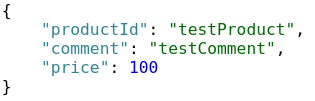
\includegraphics[height=30mm]{images/productInfoJSON.png}
    \end{center}
    \caption{Product Information example JSON}
\end{figure}

The setup of each example is described in detail in their respective repositories included in the Appendex B. Generally, each service is a standalone Java application that must run in a separated terminal instance by default located on the local computer address (localhost). Except for the LRA example, all examples are also able to run on the Docker\cite{docker} platform using the Docker compose project\cite{docker_compose}.

Every saga invocation is asynchronous - the REST call for the order request directly returns an order identification number in the response. All of the following interactions are documented in individual services by messages that are logged by the underlying platform. The overall saga process can be examined in the \texttt{order-service} or in the case of LRA in the \texttt{api-gateway} modules.

Users are also allowed to query the persisted saga information (orders, shipments and invoices) by the respective REST endpoints described in the Appendix B. For the CQRS based examples this information is available at the \texttt{query-service} microservice, otherwise each service is expected to be responsible for maintaining its individual persistence solution which corresponds with the microservices pattern definition.

\section{The saga model}

The saga pattern used in this application is able to create orders. The order saga consists of three parts -- the production of a shipping and an invoice information and if both invocations are successful, the actual order creation. If any part of the processing fails, the whole progress is expected to be undone. For instance, if the shipment is successfully created but the invoice assembly is not able to be confirmed, the persisted shipment information as well as the order must be canceled (also optionally notifying the user that the order cannot be created). The graphical representation of the saga progress is available in the figure 6.2.

\begin{figure}
    \begin{center}
        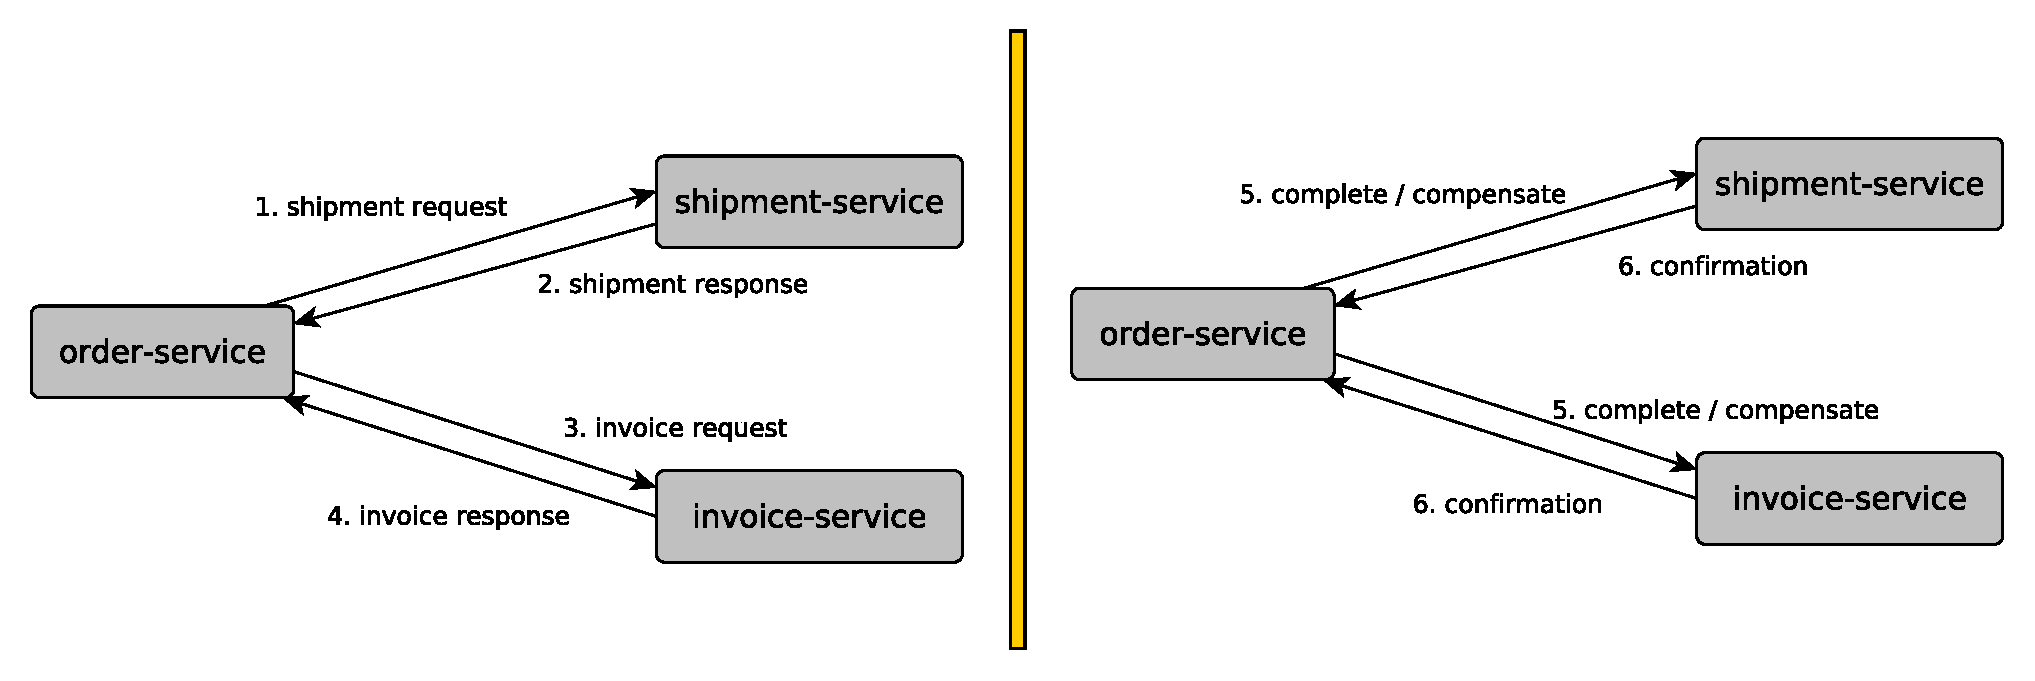
\includegraphics[height=40mm]{images/sagaModel.pdf}
    \end{center}
    \caption{The saga model}
\end{figure}

Every application is able to demonstrate three testing scenarios: the valid pass, the shipment failure and the invoice failure. In the valid scenario after the order is requested, the saga propagation invokes requests for the shipment and the invoice. If the connection between services is stable, both participants successfully return a stub answer and the order is completed. 

As most of the applied platforms invoke participants in the synchronous way, we distinguish separated member failures of the shipment or invoice. The shipment failure simulates the termination of saga without the full request coverage. This means that the compensations are distributed to all services including the \texttt{invoice-service} which has not received the work request for the order being processed yet. The scenario demonstrates the need of microservices to be able to react to the requests which are not associated with any saga which means actively keeping track of the sagas being currently executed. 

The invoice failure scenario on the other hand validates that the saga compensations are executed on all participating services as the shipment is already expected to be completed. Generally, the saga pattern assumes that the compensations of the participants are called in the reverse order of the invocations because of the possible dependencies between them.

To initiate the failures scenarios in examples both \texttt{shipment-service} and \texttt{invoice-service} are equipped with injected failure conditions. To invoke the failure the quickstarts expect a product information containing a specialized product identification: \texttt{fail-shipment} or \texttt{fail-invoice} respectively. 

The graphical representation in form of the sequence diagrams for corresponding scenarios is available in the Appendix C.

\section{Axon service}

As it was stated in the previous chapter, the Axon framework is based upon the CQRS principles. Because of this nature, it would be difficult not to follow this pattern. The individual services contain separated aggregates\footnote{for the definition of aggregate please refer to the Appendix A} each processing its respective commands and producing various events. Any inter-service interaction is restricted to the use of the command and event buses.

\subsection{Platform}

Axon service is a Java Spring Boot microservices application. Each service is fully separated and independent Maven\cite{maven} project. Every project is standalone runnable application (fat jar\footnote{Java Archive}) as the Spring Boot does not use any underlying platform to run microservices.

As a CQRS based quickstart, Axon service uses two different and separated communication channels to exchange information between services: the command bus and the event bus. By default, the Axon framework reduce both channels to one JVM\footnote{Java Virtual Machine} thus one microservice. Except from that, developers are able to specify several specialized ways of the configuration to distribute messages between different services which is used in this Axon quickstart.

The quickstart uses a motion of the distributed command bus which is based upon different approach then traditional single JVM command bus. The distributed command bus forms a bridge between separated command bus implementations to transfer commands between different JVMs. It is responsible for the selection of the communication protocol and the choice of the target destination for each incoming command.

\subsection{Structure}

The application is separated into four microservices -- the \newline \texttt{order-service}, the \texttt{shipment-service}, the \texttt{invoice-service} and the \texttt{query-service}. Furthermore it also contains a project \texttt{service-model} which serves as a support library for the microservices.



\clearpage
\chapter{Conclusion}



\makeatletter\thesis@blocks@clear\makeatother
\phantomsection %% Print the index and insert it into the
\addcontentsline{toc}{chapter}{Bibliography} %% table of contents.
\printindex

\bibliographystyle{IEEEtran}
\bibliography{IEEEabrv,references}

\appendix %% Start the appendices.

\chapter{The Command Query Responsibility Segregation pattern}

CQRS

\chapter{The example applications public APIs}

\section{Axon service}

\textbf{Order service}

\begin{minted}{python}
        POST /api/order
\end{minted}

\noindent
\textbf{Query service}

\begin{minted}{python}
        GET /api/orders
        GET /api/order/{order_id}
        GET /api/shipments
        GET /api/shipment/{shipment_id}
        GET /api/invoices
        GET /api/invoice/{invoice_id}
\end{minted}

\section{Eventuate service}

\textbf{Order service}

\begin{minted}{python}
        POST /api/order
        POST /management/shipment
        POST /management/shipment/fail
        POST /management/shipment/compensation
        POST /management/invoice
        POST /management/invoice/fail
        POST /management/invoice/compensation
\end{minted}

\noindent
\textbf{Shipment service}

\begin{minted}{python}
        POST /api/request
        POST /api/compensate
\end{minted}

\noindent
\textbf{Invoice service}

\begin{minted}{python}
        POST /api/request
        POST /api/compensate
\end{minted}

\noindent
\textbf{Query service}

\begin{minted}{python}
        GET /api/orders
        GET /api/order/{order_id}
        GET /api/shipments
        GET /api/shipment/{shipment_id}
        GET /api/invoices
        GET /api/invoice/{invoice_id}
\end{minted}

\section{LRA service}

\textbf{Order service}

\begin{minted}{python}
        POST /api/order
        GET  /api/health
\end{minted}

\noindent
\textbf{Shipment service}

\begin{minted}{python}
        POST /api/request
        PUT  /api/complete
        PUT  /api/compensate
        GET  /api/health
\end{minted}

\noindent
\textbf{Invoice service}

\begin{minted}{python}
        POST /api/request
        PUT  /api/complete
        PUT  /api/compensate
        GET  /api/health
\end{minted}

\noindent
\textbf{LRA coordinator}

\begin{minted}{python}
        GET  /lra-coordinator
        GET  /lra-coordinator/{LraId}
        GET  /lra-coordinator/status/{LraId}
        POST /lra-coordinator/start
        PUT  /lra-coordinator/{LraId}/renew
        GET  /lra-coordinator/{NestedLraId}/status
        PUT  /lra-coordinator/{NestedLraId}/complete
        PUT  /lra-coordinator/{NestedLraId}/compensate
        PUT  /lra-coordinator/{NestedLraId}/forget
        PUT  /lra-coordinator/{LraId}/close
        PUT  /lra-coordinator/{LraId}/cancel
        PUT  /lra-coordinator/{LraId}
        PUT  /lra-coordinator/{LraId}/remove
        GET  /api/health
        GET  /lra-recovery-coordinator/{LRAId}/{RecCoordId}
        PUT  /lra-recovery-coordinator/{LRAId}/{RecCoordId}
        GET  /lra-recovery-coordinator/recovery
\end{minted}

\noindent
\textbf{API gateway}

\begin{minted}{python}
        PUT  /api/complete
        PUT  /api/compensate
        GET  /api/health
        POST /api/lra
\end{minted}


\section{Eventuate Tram}

\textbf{Order service}

\begin{minted}{python}
        POST /api/order
        GET  /api/orders
        GET  /api/order/{orderId}
\end{minted}

\noindent
\textbf{Shipment service}

\begin{minted}{python}
        GET /api/shipments
        GET /api/shipment/{shipmentId}
\end{minted}

\noindent
\textbf{Invoice service}

\begin{minted}{python}
        GET /api/invoices
        GET /api/invoice/{invoiceId}
\end{minted}




\chapter{The saga scenarios}


\end{document}
